Seja \(f[a,b]\longrightarrow\mathbb{R}\) contínua, F é a prmitiva de f.
\[
  \int_{a}^{b}\,f(x)\,dx=F\big|_a^b=F(b)-F(a)
\]

\begin{definition}
Seja $P$ uma partição de $[a,b]$ que subdivide o intervalo em $n$ subintervalos

$[x_{i-1},x_i]$ de mesmo comprimento 
\[
  \Delta x = \frac{b-a}{n}.
\]
\end{definition}

\begin{theorem} (TMV -- Teorema do Valor Médio.)\label{TVM}
  Se $f$ é contínua no intervalo fechado $[a,b]$ e derivável no intervalo aberto $(a, b)$, então existe pelo menos um número $c \in (a, b)$ tal que:
\[
f'(c) = \frac{f(b) - f(a)}{b - a}
\]
\end{theorem}

Aplicando o TVM \ref{TVM} acima à função \(F\, \text{em}\, (x_{i-1}, x_{i})\exists \quad c_i \quad]\, x_{x-1,x_i \,[}\) tal que
\[
  \sum_{i=1}^{n}\,F_{x_i}-F_{(x-1,x_i)}=\sum_{i=1}^{n}f(c_i)\Delta x = F(b)-F(a)=\int_{a}^{b}f(x)\,dx
\]

Mais uma vez, seja \(f[a,b]\longrightarrow\mathbb{R}\) contínua, F é a prmitiva de f.
\[
  \int_{a}^{x}\,f(t)\,dt\,\text{é primitiva de}\,f
\]
ou seja, 
\[
  \frac{dF(x)}{dx}=\frac{d}{dx}\,\int_{a}^{x}f(t)\,dt=f(x)
\]
\begin{figure}[H]
  \centering
  \begin{tikzpicture}
    \begin{axis}[
      clip=false,
      axis x line=middle,
      axis y line=middle,
      axis line style={-{Stealth[length=3mm,width=1.5mm]}},
      xmin=0, xmax=2*pi,
      ymin=-0.5, ymax=1.2, % <- se quiser zoom, use ymin=-0.05 em vez de 0.4
      grid=both,
      ytick={0.25, .5, .75, 1},
      xtick=\empty,
      %{0,pi/2,pi,3*pi/2,2*pi}
      xticklabels=\empty, 
      % {$0$,$\frac{\pi}{2}$,$\pi$,$\frac{3\pi}{2}$,$2\pi$}
    ]

      % Curva
      \addplot[
        thick, blue, samples=200,
        domain=pi/2:3*pi/2,
        name path=curva
      ] {sin(deg(0.5*x))};

      % Caminho do eixo x (y=0) para o fillbetween
      \path[name path=xaxis] (axis cs:{pi/2},0) -- (axis cs:{3*pi/2},0);

      % Linhas verticais pontilhadas
      \draw[blue, thick, dashed] (axis cs:{pi/2},0) -- (axis cs:{pi/2},{sqrt(2)/2});
      \draw[blue, thick, dashed] (axis cs:{1.5*pi/2},0)   -- (axis cs:{1.5*pi/2},0.923);
      \draw[blue, thick, dashed] (axis cs:{3*pi/2},0) -- (axis cs:{3*pi/2},{sqrt(2)/2});

      % Área preenchida só de pi/2 até pi
      \addplot[fill=gray!35, draw=none, opacity=.5]
        fill between[of=curva and xaxis, soft clip={domain=pi/2:1.5*pi/2}];
      \node[anchor=north, yshift=-2pt] at (axis cs:{pi/2},0) {$a$};
      \node[anchor=north, yshift=-2pt] at (axis cs:{1.5*pi/2},0) {$x$};
      \node[anchor=north, yshift=-2pt] at (axis cs:{3*pi/2},0) {$b$};
    \end{axis}
  \end{tikzpicture}
\end{figure}
\newpage
\[
  \int_{a}^{x}f(t)\,dt
\]
\begin{example}
\begin{align*}
\frac{d}{dx}F(x),\quad \text{se}\quad F(x) &= \int_{1}^{x}(t^2+2)\,dt.\\
&=\frac{d}{dx}\,F(x)=X^2+2\\
\end{align*}
\end{example}

\begin{example}
  \begin{align*}
    &\frac{dy}{dx}\,\quad\text{se}\quad y=\int_{3}^{x^2}(5t+8)^{32} \,dt\\
    \text{Pela regra da cadeia}&\quad\frac{dy}{dx}=(5x^2+8)^{32}\cdot2x\\
    &y=F(u(x)),\\
    \text{onde}&\quad u(x)=x^2\quad \text{e}\quad \int_{3}^{u} (5t+8)^{32}\,dt\\
    &\frac{dy}{dx}=\frac{dF}{du}\frac{du}{dx}=(5x^2+8)^{32}\cdot 2x.
  \end{align*}
\end{example}

\begin{example}
      \begin{align*}
        \frac{d}{dx}\int_{1}^{x^4}\sec(t)\,dt=\sec(x^4)\cdot 4x^3
      \end{align*}
\end{example}


  Propriedades: se \(f\) é contínua em \([a,b]\), então:
  \begin{enumerate}
    \item 
    \[
      \int_{a}^{a}f(x)dx=0;
    \]
    \item 
    \[
      \int_{b}^{a}f(x)dx=-\int_{a}^{b}dx
    \]
  \end{enumerate}

\begin{example}
Calcule $\dfrac{dy}{dx}$, supondo $a$ constante, se
\[
y(x)=\int_{-x}^{a}\sqrt{t^{2}+1}\,dt+\int_{1}^{5x-7}\sqrt{t^{2}-1}\,dt,
\qquad (5x-7\ge 1).
\]

Usaremos a regra de Leibniz:
\[
\frac{d}{dx}\left(\int_{\alpha(x)}^{\beta(x)} f(t)\,dt\right)
= f(\beta(x))\,\beta'(x)-f(\alpha(x))\,\alpha'(x).
\]

\begin{enumerate}[label=\alph*)]
\item Para $y_1(x)=\displaystyle\int_{-x}^{a}\sqrt{t^{2}+1}\,dt$,
temos $\alpha(x)=-x$ e $\beta(x)=a$ (constante). Logo,
\[
y_1'(x)=\sqrt{a^2+1}\cdot 0-\sqrt{(-x)^2+1}\cdot(-1)=\sqrt{x^2+1}.
\]

\item Para $y_2(x)=\displaystyle\int_{1}^{5x-7}\sqrt{t^{2}-1}\,dt$,
temos $\alpha(x)=1$ (constante) e $\beta(x)=5x-7$. Então,
\[
y_2'(x)=\sqrt{(5x-7)^2-1}\cdot 5-\sqrt{1^2-1}\cdot 0
=5\sqrt{(5x-7)^2-1}.
\]

\item Portanto,
\[
\boxed{\frac{dy}{dx}=\sqrt{x^2+1}+5\sqrt{(5x-7)^2-1}},
\qquad \text{válido para } 5x-7\ge 1 \ (x\ge 8/5).
\]
\end{enumerate}
\end{example}

\section{Derivada de Integrais com Limites Variáveis}

\subsection{1. Interpretação Geométrica}

Considere
\[
F(x)=\int_{0}^{x} f(t)\,dt.
\]

A função $F(x)$ representa a área acumulada sob o gráfico de $f(t)$
desde $0$ até $x$.

Quando $x$ aumenta para $x+h$, a nova área acumulada é

\[
F(x+h)=\int_{0}^{x+h} f(t)\,dt.
\]

Logo,

\[
F(x+h)-F(x)=\int_{x}^{x+h} f(t)\,dt.
\]

Essa diferença corresponde à pequena faixa adicionada no final do intervalo.

\subsubsection*{Ilustração Geométrica}

\begin{figure}[H]
\centering
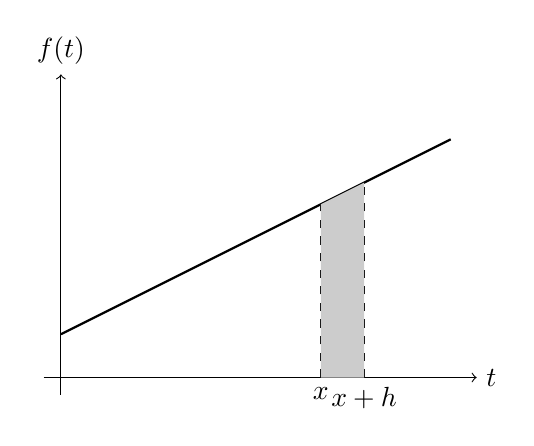
\begin{tikzpicture}[scale=1.1]

% Eixos
\draw[->] (-0.2,0) -- (4.8,0) node[right] {$t$};
\draw[->] (0,-0.2) -- (0,3.5) node[above] {$f(t)$};

% Curva
\draw[domain=0:4.5,smooth,variable=\x,thick]
plot ({\x},{0.5*\x+0.5});

% Pontos x e x+h
\draw[dashed] (3,0) -- (3,2);
\draw[dashed] (3.5,0) -- (3.5,2.25);

\node[below] at (3,0) {$x$};
\node[below] at (3.5,0) {$x+h$};

% Área pequena
\fill[gray!40] (3,0) -- (3,2) -- (3.5,2.25) -- (3.5,0) -- cycle;

\end{tikzpicture}
\caption{A pequena faixa de área adicionada quando $x$ varia para $x+h$.}
\end{figure}

Se $h$ é pequeno, essa área é aproximadamente um retângulo de:

\[
\text{altura } \approx f(x),
\qquad
\text{largura } = h.
\]

Assim,

\[
F(x+h)-F(x)\approx f(x)\,h.
\]

Dividindo por $h$ e passando ao limite:

\[
\boxed{F'(x)=f(x).}
\]

\subsection{2. Demonstração Formal}

Considere

\[
F(x)=\int_{0}^{x} f(t)\,dt.
\]

Pela definição de derivada:

\[
F'(x)=\lim_{h\to 0}
\frac{F(x+h)-F(x)}{h}.
\]

Mas:

\[
F(x+h)-F(x)=\int_{x}^{x+h} f(t)\,dt.
\]

Pelo Teorema do Valor Médio para integrais, existe
$c\in[x,x+h]$ tal que

\[
\int_{x}^{x+h} f(t)\,dt = f(c)\,h.
\]

Logo,

\[
\frac{F(x+h)-F(x)}{h}=f(c).
\]

Quando $h\to 0$, temos $c\to x$, e como $f$ é contínua:

\[
F'(x)=f(x).
\]

\subsection{3. Caso com Limite Variável Geral}

Se

\[
F(x)=\int_{0}^{g(x)} f(t)\,dt,
\]

então:

\[
F'(x)=f(g(x))\,g'(x).
\]

Aqui aparece naturalmente a regra da cadeia.

\subsection{4. Regra Geral (Regra de Leibniz)}

Se ambos os limites dependem de $x$:

\[
F(x)=\int_{\alpha(x)}^{\beta(x)} f(t)\,dt,
\]

então:

\[
\boxed{
F'(x)
=
f(\beta(x))\,\beta'(x)
-
f(\alpha(x))\,\alpha'(x).
}
\]

\subsection{Interpretação}

\begin{itemize}
    \item O limite superior adiciona área.
    \item O limite inferior remove área.
    \item O sinal negativo surge da orientação do intervalo.
\end{itemize}

\subsection{5. Exemplo Completo}

Considere

\[
y(x)=\int_{-x}^{a}\sqrt{t^2+1}\,dt,
\quad a \text{ constante}.
\]

Temos:

\[
\alpha(x)=-x,
\qquad
\beta(x)=a.
\]

Aplicando a regra:

\[
y'(x)
=
\sqrt{a^2+1}\cdot 0
-
\sqrt{(-x)^2+1}\cdot(-1).
\]

Logo,

\[
\boxed{y'(x)=\sqrt{x^2+1}.}
\]

\subsection{Resumo Final}

\[
\boxed{
\frac{d}{dx}
\left(
\int_{\alpha(x)}^{\beta(x)} f(t)\,dt
\right)
=
f(\beta(x))\beta'(x)
-
f(\alpha(x))\alpha'(x)
}
\]

Esta fórmula resolve todos os exercícios desse tipo.


\subsection{Exemplos clássicos}

\begin{itemize}
  \item \(f(x)=x\) em \([0,1]\): contínua \(\Rightarrow\) integrável e 
  \[
  \int_0^1 x\,dx = \frac{x^2}{2}\Bigg|_0^1=\frac{1}{2}
  \].
  \item \textbf{Dirichlet:} \(f(x)=1\) se \(x\) é racional e \(0\) se irracional em \([0,1]\). Não é integrável no sentido de Riemann.
  \item \textbf{Thomae ("pipoca"):} 
  \(f(x)=\begin{cases}1/q, & x=p/q
    \ (\gcd(p,q)=1)\\[2pt] 0, & x\ \text{irracional}\end{cases}\).

    É integrável no sentido de Riemann e 
    \[
      \int_0^1 f\,dx = 0.
    \]
\end{itemize}

\subsubsection{Exemplo por somas superior/inferior}
Para \(f(x)=x\) em \([0,1]\), use a partição uniforme \(x_i=i/n\).
Temos \(m_i=x_{i-1}=\tfrac{i-1}{n}\) e \(M_i=x_i=\tfrac{i}{n}\). Logo,
\[
L(P_n,f)=\sum_{i=1}^n \frac{i-1}{n}\cdot\frac{1}{n}
=\frac{1}{n^2}\sum_{k=0}^{n-1}k
=\frac{n-1}{2n},
\]
\[
U(P_n,f)=\sum_{i=1}^n \frac{i}{n}\cdot\frac{1}{n}
=\frac{1}{n^2}\sum_{i=1}^{n}i
=\frac{n+1}{2n}.
\]
Como \(L(P_n,f), U(P_n,f) \to \tfrac{1}{2}\), conclui-se que \(\displaystyle 
\int_0^1 x\,dx = \tfrac{1}{2}\).

\subsubsection{Relação do TFC com as integrais definidas}
Se \(F\) é uma primitiva de \(f\) (\(F'=f\)), então:
\[
\int_a^b f(x)\,dx = F(b)-F(a).
\]

\subsubsection{Integrais impróprias (observação)}
Se \(f\) não é limitada em \([a,b]\) ou se o intervalo é infinito, define-se por limites:
\[
\int_a^b f(x)\,dx
=\lim_{t\to b^-}\int_a^t f(x)\,dx,\qquad
\int_a^{+\infty} f(x)\,dx
=\lim_{t\to +\infty}\int_a^{t} f(x)\,dx.
\]

\subsubsection{Propriedades úteis}
Para funções integráveis \(f, g\) e escalares \(\alpha, \beta\):
\begin{align*}
&\int_a^b (\alpha f + \beta g)\,dx = \alpha\int_a^b f\,dx + \beta\int_a^b g\,dx,\\
&\int_a^b f\,dx = \int_a^c f\,dx + \int_c^b f\,dx,\\
&\int_a^b f\,dx = -\int_b^a f\,dx.
\end{align*}

\[
f: [a,b] \to \mathbb{R}, \quad f \geq 0
\]

\begin{figure}[H]
  \centering
  \begin{tikzpicture}
    \begin{axis}[
      xmin=0.5, xmax=3,
      ymin=0.6, ymax=1.1,
      axis x line=middle,
      axis y line=middle,
      axis line style={-{Stealth[length=3mm,width=1.5mm]}},
      tick align=outside,
      minor tick num=3,
      xlabel={$x$}, 
      ylabel={$y$},
      xlabel style={at={(axis description cs:1,-0.08)},anchor=north},
      title={$f(x) = 0,9 \operatorname{sen}(0,8x)$}
    ]
      % Intervalo de sombreamento
      \def\a{1}
      \def\b{2.5}

      \addplot[name path=curva, domain=\a:\b, samples=250, thick]
        {0.9*sin(deg(0.8*x))};
      \addplot[name path=base, domain=\a:\b, samples=2] {0};

      \addplot[fill=gray!20, draw=none, opacity=.5]
        fill between[of=curva and base];

      \draw[line width=0.6pt] (axis cs:\a,0) -- (axis cs:\a,{0.9*sin(deg(0.8*\a))});
      \draw[line width=0.6pt] (axis cs:\b,0) -- (axis cs:\b,{0.9*sin(deg(0.8*\b))});
    \end{axis}
  \end{tikzpicture}
  \caption{Área sob o gráfico.}
\end{figure}

Se, por hipótese, deseja-se calcular a área sob a curva, calcula-se a integral da função entre os limites de integração $[a,b]$, ou seja, a integral de Riemann.
\medskip
 
A área de \(S\) é:
\[
\int_a^b f(x)\,dx = \lim_{\|\Delta x\| \to 0} \sum_{i=1}^n f(c_i )(x_i - x_{i-1}).
\]

Seja \(f:[a,b] \to \mathbb{R}\) contínua. Se \(F\) é uma primitiva de \(f\), então:
\[
\int_{a}^{b}f(x)\,dx = F(x)\Big|_{a}^{b} = F(b)-F(a).
\]

\begin{exercicio}\label{ex:int_x2_0_5}
Calcule a integral definida:
\begin{align*}
\int_{0}^{5}x^2\,dx
&= \frac{x^3}{3}\bigg|_{0}^{5}\\
&= \frac{5^3}{3} - \frac{0^3}{3}\\
&= \boxed{\frac{125}{3}\,u.a.}
\end{align*}
\end{exercicio}

\begin{exercicio}\label{ex:int_e_-1_1_}
Calcule a integral definida:
\begin{align*}
 &\int_{-1}^{1}e^x\,dx = e^x\bigg|_{-1}^{1}\\
 &= e^1 - e^{-1}\\
 &= \boxed{e - \frac{1}{e}}\,u.a.
\end{align*}
\end{exercicio}

\begin{exercicio}\label{int_x2_-2a}
  Calcule a integral definida:
 \begin{align*}
    &\int_{0}^{2}(x^2 - 2x)\,dx\\
    &= \int_{0}^{2}x^2\,dx - 2\int_{0}^{2}x\,dx \\
    &= \frac{x^3}{3}\bigg|_{0}^{2} - x^2\bigg|_{0}^{2} \\
    &= \frac{8}{3} - 4 = \boxed{-\frac{4}{3}}\,u.a.
\end{align*}
\end{exercicio}

\begin{exercicio}\label{int_4x_x2}
  Calcule a Intedgral definida:
  \begin{align*}
    & \int_{2}^{4}(4x-x^2)  \,dx \\
    &=\Big[2x^2-\frac{x^3}{3}\Big]_2^4\\
    &=(2\cdot 4^2-\frac{4^3}{3})-(2\cdot 2^2-\frac{2^3}{3})\\
    &=\Big(32-\frac{64}{3}\Big)-\Big(8-\frac{8}{3}\Big)\\
    &=\frac{32}{3}-\frac{16}{3}= \boxed{\frac{16}{3}}
  \end{align*}
\end{exercicio}
    
\begin{figure}[H]
  \centering
  \begin{tikzpicture}
    \begin{axis}[
      xmin=-0.5, xmax=3,
      ymin=-1.5, ymax=2,
      axis x line=middle,
      axis y line=middle,
      axis line style={-{Stealth[length=3mm,width=1.5mm]}},
      xlabel={$x$},
      ylabel={$y$},
    ]
      \addplot[red, domain=-0.5:2.5, samples=200, thick] {x^2-2*x};
      \addplot[domain=0:2, samples=200, draw=none, fill=gray!20, opacity=.35] {x^2-2*x} \closedcycle;
    \end{axis}
  \end{tikzpicture}
  \caption{Função $f(x)=x^2-2x$ e a área (abaixo do eixo $x$).}
\end{figure}

\subsubsection{O Teorema Fundamental do Cálculo (Parte 1)}

O TFC estabelece que a derivada de uma função definida por uma integral é o próprio integrando avaliado no limite de integração superior. Quando o limite superior é uma função $g(x)$, aplicamos a Regra da Cadeia:

\[ 
\frac{d}{dx} \int_{a}^{g(x)} f(t) \, dt = f(g(x)) \cdot g'(x)
\]

\begin{exercicio}
      Encontre a derivada da função:
      \[
        F(x) = \int_{3}^{x^2} \ln(t + 1) \, dt.
      \]
      \medskip
      \begin{enumerate}[label=\alph*.]
        \item Identificamos o integrando $f(t) = \ln(t + 1)$ e o limite superior $g(x) = x^2$.
        \item Substituímos $t$ por $g(x)$ na função:
        $$f(g(x)) = \ln(x^2 + 1)$$
        \item Multiplicamos pela derivada de $g(x)$, sendo 
              \begin{align*}
                &g'(x) = 2x:\\
                &F'(x) = \ln(x^2 + 1) \cdot 2x\\
          \end{align*}
      \end{enumerate}
      \[
      F'(x) = 2x \ln(x^2 + 1)
      \]
\end{exercicio}

\subsubsection{Caso Geral -- Ambos os limites são funções}

Se a função possui variáveis em ambos os limites de integração:
\[
  F(x) = \int_{h(x)}^{g(x)} f(t) \, dt
\]
A derivada é dada por:
  \[
    F'(x) = f(g(x)) \cdot g'(x) - f(h(x)) \cdot h'(x)
  \]
  \begin{exercicio}
    Seja \(f(x)=x^2-4\) e \(g(x)=(-x^2-2x)\) calcule a área sob as curvas entre os limites [-3,0]

    \begin{figure}[H]
  \centering
      \begin{tikzpicture}
          \begin{axis}[
            xmin=-3.5, xmax=0.5,
            ymin=0, ymax=5.5,
            axis x line=middle,
            axis y line=middle,
            axis line style={-{Stealth[length=3mm,width=1.5mm]}},
            xlabel={$x$},
            ylabel={$y$},
                ]
            \addplot[red, domain=-3:-2, samples=200, thick] {x^2-4};
            \addplot[blue, domain=-2.5:0, samples=200, thick] {-x^2-2*x};
            \draw[azulmarinho, dashed] (-3,0) -- (-3,5);
            \addplot[domain=-3:-2, samples=200, draw=none, fill=gray!20, opacity=.35] {x^2-4} \closedcycle;
            \addplot[domain=-2:0, samples=200, draw=none, fill=gray!20, opacity=.35] {-x^2-2*x} \closedcycle;
          \end{axis}
      \end{tikzpicture}
  \caption{Função $f(x)=x^2-4$ e $g(x)=-x^2-2x$.}
\end{figure}
\begin{align*}
    &\text{Primeira Integral}\\
    &\int_{-3}^{-2}(x^2-4)\,dx\\
    &=\Bigg[\frac{x^3}{3}-4x\Bigg]_{-3}^{-2}\\
    &= \Bigg[\frac{(-2)^3}{3}-(4\cdot(-2))\Bigg]-\Bigg[\frac{(-3)^3}{3}-(4\cdot(-3))\Bigg]\\
    &-\frac{8}{3}-(-8)-(-\frac{27}{3}-(-12))\\
    &-\frac{8}{3}+\frac{24}{3}-\Big(-\frac{27}{3}+\frac{36}{3}\Big)\\
    &\frac{16}{3}-\frac{9}{3}=\frac{7}{3}\\\\
    &\text{Segunda Integral}\\
    &\int_{-2}^{0}(-x^2-2x)\,dx\\
    &\Bigg[\Big(-\frac{x^3}{3}\Big)-\Big(x^2\Big)\Bigg]_{-2}^0\\
    &0-\Bigg[\Big(-\frac{-2^3}{3}\Big)-\Big(-2^2\Big)\Bigg]\\
    &0-\Big(\frac{8}{3}-4\Big)=0-\Big(-\frac{4}{3}\Big)=\frac{4}{3}\\\\
    &\text{Área total}\\
    &\frac{7}{3}+\frac{4}{3}=\boxed{\frac{11}{3}}\,\text{u.a.}
\end{align*}
  \end{exercicio}

